% Options for packages loaded elsewhere
\PassOptionsToPackage{unicode}{hyperref}
\PassOptionsToPackage{hyphens}{url}
%
\documentclass[
]{article}
\usepackage{lmodern}
\usepackage{amsmath}
\usepackage{ifxetex,ifluatex}
\ifnum 0\ifxetex 1\fi\ifluatex 1\fi=0 % if pdftex
  \usepackage[T1]{fontenc}
  \usepackage[utf8]{inputenc}
  \usepackage{textcomp} % provide euro and other symbols
  \usepackage{amssymb}
\else % if luatex or xetex
  \usepackage{unicode-math}
  \defaultfontfeatures{Scale=MatchLowercase}
  \defaultfontfeatures[\rmfamily]{Ligatures=TeX,Scale=1}
\fi
% Use upquote if available, for straight quotes in verbatim environments
\IfFileExists{upquote.sty}{\usepackage{upquote}}{}
\IfFileExists{microtype.sty}{% use microtype if available
  \usepackage[]{microtype}
  \UseMicrotypeSet[protrusion]{basicmath} % disable protrusion for tt fonts
}{}
\makeatletter
\@ifundefined{KOMAClassName}{% if non-KOMA class
  \IfFileExists{parskip.sty}{%
    \usepackage{parskip}
  }{% else
    \setlength{\parindent}{0pt}
    \setlength{\parskip}{6pt plus 2pt minus 1pt}}
}{% if KOMA class
  \KOMAoptions{parskip=half}}
\makeatother
\usepackage{xcolor}
\IfFileExists{xurl.sty}{\usepackage{xurl}}{} % add URL line breaks if available
\IfFileExists{bookmark.sty}{\usepackage{bookmark}}{\usepackage{hyperref}}
\hypersetup{
  pdftitle={Maintainance of Certification and Medicare Outcomes},
  pdfauthor={Xilin Chen},
  hidelinks,
  pdfcreator={LaTeX via pandoc}}
\urlstyle{same} % disable monospaced font for URLs
\usepackage[margin=1in]{geometry}
\usepackage{graphicx}
\makeatletter
\def\maxwidth{\ifdim\Gin@nat@width>\linewidth\linewidth\else\Gin@nat@width\fi}
\def\maxheight{\ifdim\Gin@nat@height>\textheight\textheight\else\Gin@nat@height\fi}
\makeatother
% Scale images if necessary, so that they will not overflow the page
% margins by default, and it is still possible to overwrite the defaults
% using explicit options in \includegraphics[width, height, ...]{}
\setkeys{Gin}{width=\maxwidth,height=\maxheight,keepaspectratio}
% Set default figure placement to htbp
\makeatletter
\def\fps@figure{htbp}
\makeatother
\setlength{\emergencystretch}{3em} % prevent overfull lines
\providecommand{\tightlist}{%
  \setlength{\itemsep}{0pt}\setlength{\parskip}{0pt}}
\setcounter{secnumdepth}{-\maxdimen} % remove section numbering
\usepackage{booktabs}
\usepackage{longtable}
\usepackage{array}
\usepackage{multirow}
\usepackage{wrapfig}
\usepackage{float}
\usepackage{colortbl}
\usepackage{pdflscape}
\usepackage{tabu}
\usepackage{threeparttable}
\usepackage{threeparttablex}
\usepackage[normalem]{ulem}
\usepackage{makecell}
\usepackage{xcolor}
\ifluatex
  \usepackage{selnolig}  % disable illegal ligatures
\fi

\title{Maintainance of Certification and Medicare Outcomes}
\usepackage{etoolbox}
\makeatletter
\providecommand{\subtitle}[1]{% add subtitle to \maketitle
  \apptocmd{\@title}{\par {\large #1 \par}}{}{}
}
\makeatother
\subtitle{Cohort Definition}
\author{Xilin Chen}
\date{2021-05-19}

\begin{document}
\maketitle

{
\setcounter{tocdepth}{3}
\tableofcontents
}
This document describes how the ABS maintenance of certification and
medicare outcomes cohort was defined. The data will be used for further
statistical analyses.

\hypertarget{data-sources}{%
\subsection{1. Data Sources}\label{data-sources}}

\begin{itemize}
\tightlist
\item
  ABS certification data (received at September 2019 from ABS)
\item
  Medicare claim data

  \begin{itemize}
  \tightlist
  \item
    Year: 2007-2018
  \item
    Procedures: commonly performed general surgery procedures (162
    procedures in total)
  \end{itemize}
\end{itemize}

ABS and Medicare claim data are linked using physician NPIs.

\pagebreak

\hypertarget{cohort-definition-diagram-overview}{%
\subsection{2. Cohort definition diagram
overview}\label{cohort-definition-diagram-overview}}

Below is the consort diagram for the data selection process. Detailed
cohort selection descriptions are included in \emph{3. Data Process} and
\emph{4. Data linkage}.

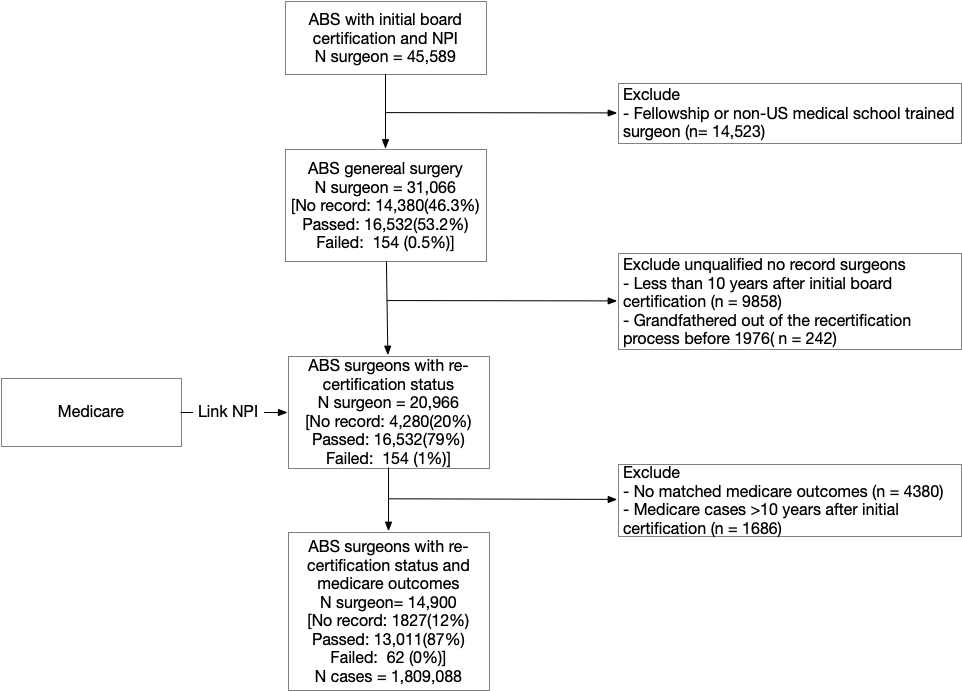
\includegraphics{/Users/xilinchen/Documents/Repo/ABS_MoC_vs_pt_Outcome/other_docs/Diagram/cohort_definition/cohort_definition.png}

\hypertarget{data-process}{%
\subsection{3. Data Process}\label{data-process}}

\hypertarget{abs}{%
\subsubsection{ABS}\label{abs}}

\hypertarget{inclusion-and-exclusion}{%
\subsubsection{3.1. Inclusion and
Exclusion}\label{inclusion-and-exclusion}}

Inclusion:

\begin{itemize}
\tightlist
\item
  Surgeons with NPI
\item
  Passed initial certification exam
\item
  Not qualified (10 years after initial certification) for exam after
  2017 (exam change in 2017)

  \begin{itemize}
  \tightlist
  \item
    to address the exam changes in 2017, we excluded all surgeons who
    were qualified for recertification after(including) 2017. In our
    dataset, we don't have the recertifcation exam years for surgeons.
    So it's not possible to know if the surgeon took the exam before or
    after 2017. By excluding surgeons who were qualified to take the
    exam after 2017, we exclude the group who might have taken the exam
    after 2017. However, this also excluded some surgeons who took
    recertification exam earlier than 10 years after the initial
    certification.
  \end{itemize}
\end{itemize}

Exclusion:

\begin{itemize}
\tightlist
\item
  Fellowship or non-US trained surgeons (n = 14523).

  \begin{itemize}
  \tightlist
  \item
    Fellowship and Med school information is from ABS, AMA and
    Fellowship Council data.
  \end{itemize}
\end{itemize}

Below is the re-certification status for all qualified ABS surgeons.
Very few surgeons have recorded failed re-certification status. A large
portion of surgeons didn't have re-certification records at all,
i.e.~NA.

\begin{table}[H]
\centering
\begin{tabular}{r|r|l}
\hline
ReCeverPassed & n suregon & percentage\\
\hline
0 & 138 & 1\%\\
\hline
1 & 15838 & 65\%\\
\hline
NA & 8511 & 35\%\\
\hline
\end{tabular}
\end{table}

\hypertarget{define-never-recertified-surgeon-group-define-na-group}{%
\subsubsection{3.2. Define never recertified surgeon group (Define NA
group)}\label{define-never-recertified-surgeon-group-define-na-group}}

\hypertarget{at-least-10-years-after-the-initial-certification-year}{%
\paragraph{3.2.1. At least 10 years after the initial certification
year}\label{at-least-10-years-after-the-initial-certification-year}}

The ABS require diplomats certified subsequently to pass a secure,
multiple-choice comprehensive recertification examination in surgery
every 10 years.

5999 surgeons who had no recertification record but had initial board
certification more than 10 years ago. We include this group as failed
recertification group. Surgeons who didn't have 10 years after the
initial certification process were excluded because they didn't have
enough time to pass the re-certification exam.

\hypertarget{grandfathered-out-of-the-recertification-process}{%
\paragraph{3.2.2 Grandfathered out of the recertification
process}\label{grandfathered-out-of-the-recertification-process}}

We excluded surgeons who had their initial certification before 1976. It
was bases on the recertification was introduced at 1976 ``the American
Board of Surgery (ABS) introduced time-limited certification in 1976,
requiring diplomats certified subsequently to pass\ldots{}''. If the
surgeon was initially certified before 1976, she/he was not required for
recertification at the initial certification time.

702 surgeons graduated before 1976 and are excluded in the analyses
cohort. Below are the surgeon re-certification status after excluding
the 10 years cutoff and grandfathered out surgeons.

\begin{table}[H]
\centering
\begin{tabular}{l|r|l}
\hline
Recert\_status & n suregon & percentage\\
\hline
failed & 138 & 1\%\\
\hline
NA\_failed & 5297 & 25\%\\
\hline
passed & 15838 & 74\%\\
\hline
\end{tabular}
\end{table}

\hypertarget{data-linkage}{%
\subsection{4. Data linkage}\label{data-linkage}}

\hypertarget{link-medicare-data-with-abs-data-by-npi}{%
\subsubsection{4.1 Link Medicare data with ABS data by
NPI}\label{link-medicare-data-with-abs-data-by-npi}}

\hypertarget{only-keep-cases-that-performed-between-10-20-years-after-initial-certification}{%
\subsubsection{4.2 Only keep cases that performed between 10-20 years
after initial
certification*}\label{only-keep-cases-that-performed-between-10-20-years-after-initial-certification}}

The ABS gives 10 years for surgeons for the recertification. We keep
cases that 10 years after the initial certification to better capture
the impact of the recertification process. However, we excluded cases
happened 20 years after the initial certification to elude the
re-recertification effect,.e. only the first recertificastion cases were
included in the cohort.

Link ABS with Medicare by NPI. Below is the number of surgeons by each
recertification category after linked with Medicare outcomes.

\begin{table}[H]
\centering
\begin{tabular}{l|r|l}
\hline
Recert\_status & n suregon & percentage\\
\hline
failed & 44 & 0\%\\
\hline
NA\_failed & 1173 & 11\%\\
\hline
passed & 9602 & 89\%\\
\hline
\end{tabular}
\end{table}

5314 ABS surgeons don't have Medicare cases matched; 5140 surgeons don't
have cases between 10 to 20 years after the initial certification.

\end{document}
